\usepackage
  [ includehead
  , top=4cm
  , bottom=5cm
  , left=4cm
  , right=4cm
  ]{geometry}
\usepackage[table]{xcolor}

\usepackage{commutative-diagrams}

\def\nope{\cellcolor{green!30}}
\def\yupe{\cellcolor{red!30}}
\definecolor{LightRed}{rgb}{0.980,0.407,0.400}
\definecolor{backgroundColor}{rgb}{1,1,1}
\definecolor{linkBrownRed}{rgb}{0.6,0.12156862745,0}
\definecolor{lightGray}{rgb}{0.8,0.8,0.8}
\definecolor{grayY}{rgb}{0.95,0.95,0.95}
\definecolor{grayN}{rgb}{1,1,1}

% Packages
\usepackage
  { amssymb
  , amsmath
  , adjustbox
  , amsthm
  , booktabs
  , lmodern
  , mathtools
  , tikz-cd
  , todonotes
  , xparse
  , proof
  , wrapfig
  , xspace
  , ytableau
  , cancel
}
\usetikzlibrary{decorations.pathmorphing}

\usepackage[utf8]{inputenc}
\usepackage[T1]{fontenc}

\ytableausetup{smalltableaux,centertableaux}

\tikzcdset{
    arrow style=tikz,
    diagrams={>={Stealth[round,length=4pt,width=4.95pt,inset=2.75pt]}}
}
\tikzset{double line with arrow/.style args={#1,#2}{decorate,decoration={markings,%
mark=at position 0 with {\coordinate (ta-base-1) at (0,1pt);
\coordinate (ta-base-2) at (0,-1pt);},
mark=at position 1 with {\draw[#1] (ta-base-1) -- (0,1pt);
\draw[#2] (ta-base-2) -- (0,-1pt);
}}}}
\tikzset{Equals/.style={-,double line with arrow={-,-}}}
\usepackage[ protrusion=true
           , expansion=true
           ]{microtype}

\usepackage
  [ maxbibnames=20 
  , backend=biber 
  , backref=true 
  , style=alphabetic 
  , citestyle=alphabetic
  ]{biblatex}
\addbibresource{./bibliography.bib}

\usepackage{hyperref}
\hypersetup{
    colorlinks,
    citecolor=linkBrownRed,
    filecolor=linkBrownRed,
    linkcolor=linkBrownRed,
    urlcolor=linkBrownRed
}

\usepackage[capitalise,nameinlink,noabbrev]{cleveref}
\renewcommand{\cref}[1]{\Cref{#1}}
\makeatletter
\def\defthm#1#2{%
  \newtheorem{#1}{#2}[section]%
  \expandafter\def\csname #1autorefname\endcsname{#2}%
  \expandafter\let\csname c@#1\endcsname\c@theorem}
\makeatother

\theoremstyle{definition}
\numberwithin{equation}{section}
\newtheorem{theorem}{Theorem}[section]
 \defthm{corollary}{Corollary}
 \defthm{proposition}{Proposition}
 \defthm{lemma}{Lemma}
 \defthm{claim}{Claim}
 \defthm{definition}{Definition}
 \defthm{notation}{Notation}
 \defthm{remark}{Remark}
 \defthm{conjecture}{Conjecture}
 \defthm{axiom}{Axiom}
 \defthm{example}{Example}
 \defthm{non-example}{Non-Example}
 \defthm{examples}{Examples}
 \defthm{exercise}{Exercise}
 \defthm{counterexample}{Counterexample}
 \defthm{construction}{Construction}
 \defthm{warning}{Warning}
 \defthm{digression}{Digression}
 \defthm{perspective}{Perspective}
 \defthm{discussion}{Discussion}
 \defthm{terminology}{Terminology}
 \defthm{heuristics}{Heuristics}

\newtheorem*{definition*}{Definition}
\newcommand{\din}{%
    \mathrel{%
        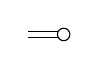
\begin{tikzpicture}[baseline=-0.58ex]
            \draw[line width=.425pt] (0,.035) -- ++(.45,0);
            \draw[line width=.425pt] (0,-.035) -- ++(.45,0);
            \draw[fill=white] (.45,.0) circle (2.25pt);
        \end{tikzpicture}
    }
}

\newcommand{\uptpl}[2]{\overset{#2 \text{ times}}{\scriptstyle #1,\dots,#1}}
\newcommand{\dwntpl}[2]{\underset{#2 \text{ times}f}{\scriptstyle #1,\dots,#1}}

\newcommand{\wlim}[1]{\mathrm{lim}^{#1}}
\newcommand{\wcolim}[1]{\mathrm{colim}^{#1}}
\newcommand{\procirc}{\mathbin{\diamond}}
\newcommand{\ph}{\mathsf{h}}
\newcommand{\pqdiag}{\Delta_{p,q}}

% \input{./preamble/arrows.tex}
% \input{./preamble/colours.tex}
% \input{./preamble/widebar.tex}
% \input{./preamble/fonts.tex}
% \input{./preamble/diagram_environment.tex}
% \input{./preamble/toc.tex}

\usepackage{CJKutf8}
\def\jap#1{\begin{CJK}{UTF8}{bsmi}#1\end{CJK}}

\newcommand{\CatFont}[1]{\mathcal{#1}}
\newcommand{\Obj}{\mathrm{Obj}}%
\newcommand{\Hom}{\mathrm{hom}}%
\newcommand{\SloganFont}[1]{{\textit{#1. }}}
\newcommand{\Cones}[2]{\mathsf{Cones}_{#1}\big(#2\big)}
\newcommand{\Wedges}[2]{\mathsf{Wd}_{#1}\big(#2\big)}
\newcommand{\Cowedges}[2]{\mathsf{CWd}_{#1}\big(#2\big)}
\newcommand{\Mor}{\mathrm{Mor}}%
\usepackage{xfrac}
\newcommand{\yn}{\sfrac{\mathrm{Y}}{\mathrm{N}}}%
\newcommand{\ynyn}[4]{[\textsc{#1}|\textsc{#2}|\textsc{#3}|\textsc{#4}]}%
\newcommand{\otimesDay}{\mathbin{\circledast}}
\renewcommand{\Vert}[1]{\mathrm{Vert}(#1)}
\newcommand{\Edges}[1]{\mathrm{Edges}(#1)}
\newcommand{\source}{\mathsf{s}}
\newcommand{\target}{\mathsf{t}}

% \newcommand{\WeightedEnd}[2]{\int_{#1}^{#2}}
% \newcommand{\WeightedCoend}[2]{\int^{#1}_{#2}}
\newcommand{\nin}{\not{\in}}
\newcommand{\Open}{\mathsf{Op}}
\newcommand{\Arr}{\mathsf{Arr}}
\newcommand{\Top}{\mathsf{Top}}
\newcommand{\Tot}{\mathrm{Tot}}
\newcommand{\sSets}{\mathsf{sSet}}
\newcommand{\Cech}{\textsf{Č}_{\bullet}}
\newcommand{\pr}{\bst}
\newcommand{\projection}{\mathrm{pr}}
\newcommand{\inj}{[\boldsymbol{0}]}
\newcommand{\col}{\mathsf{col}}
\newcommand{\point}{\star}
\newcommand{\ceiling}[1]{\lceil#1\rceil}
\let\ceil\ceiling
\newcommand{\WCC}{\mathsf{C}}
\newcommand{\ConstantP}[2]{\boldsymbol{#1}_{#2}}
\newcommand{\ConstantPNo}[2]{\boldsymbol{#1}_{#2}}% No=possibly dropable subscripts
\newcommand{\ddelta}{\boldsymbol{\delta}}
\newcommand{\smallvskip}{\par\vspace*{0.25\baselineskip}}
\newcommand{\rA}{\textcolor{red}{A}}
\newcommand{\rB}{\textcolor{red}{B}}
\newcommand{\rX}{\textcolor{red}{X}}
\newcommand{\rY}{\textcolor{red}{Y}}
\newcommand{\rf}{\textcolor{red}{f}}
\newcommand{\bX}{\textcolor{blue}{X}}
\newcommand{\bY}{\textcolor{blue}{Y}}
\newcommand{\bB}{\textcolor{blue}{B}}
\newcommand{\bC}{\textcolor{blue}{C}}
\definecolor{darkGreen}{RGB}{2,127,27}
\newcommand{\gC}{\textcolor{darkGreen}{C}}
\newcommand{\gD}{\textcolor{darkGreen}{D}}
\newcommand{\mlp}[1]{\mathllap{#1}}
\newcommand{\mcp}[1]{\mathclap{#1}}
\newcommand{\mrp}[1]{\mathrlap{#1}}
\DeclareMathOperator*{\biprod}{\sfM}%{\mathrlap{\prod}\mathrlap{\coprod}\phantom{\coprod}}
\DeclareMathOperator{\biprodnl}{\mathrlap{\prod}\mathrlap{\coprod}\phantom{\coprod}}
\DeclareMathOperator*{\prodbi}{\sfW}%{\rotatebox[origin=c]{90}{$\biprod$}}
\DeclareMathOperator{\prodbinl}{\rotatebox[origin=c]{90}{$\biprod$}}
\DeclareRobustCommand{\CatEl}[2]{#1\rotatebox[origin=c]{15}{$\int$}#2}
\newcommand{\negphantom}[1]{\settowidth{\dimen0}{#1}\hspace*{-\dimen0}}
\newcommand{\Mod}{\mathsf{Mod}}
\newcommand{\Ab}{\mathsf{Ab}}
\newcommand{\Dd}{\mathrm{d}}
\newcommand{\Z}{\mathbb{Z}}
\newcommand{\pt}{\mathrm{pt}}
\newcommand{\textiff}{iff\xspace}
\newcommand{\Tw}[1]{\mathsf{Tw}(#1)}
\newcommand{\Forgetful}{\Sigma}%{\text{¿}}%{\text{\jap{忘}}}
\newcommand{\yo}{\text{\begin{CJK}{UTF8}{min}よ\end{CJK}}}
\newcommand{\coyo}{%
    \mathchoice%
    {\rotatebox[origin=c]{180}{\yo}}
    {\rotatebox[origin=c]{180}{\yo}}
    {\rotatebox[origin=c]{180}{\scriptsize\yo}}
    {\rotatebox[origin=c]{180}{\tiny\yo}}
}
\newcommand{\unsim}{\mathord{\sim}}
\newcommand{\otimesDayN}[1]{\mathbin{\circledast}_{#1}}
\newcommand{\SimplexCategory}{\boldsymbol{\Delta}}
\newcommand{\diag}{\mathrm{diag}}
\newcommand{\ev}{\mathsf{ev}}
\newcommand{\Lan}{\mathsf{Lan}}
\newcommand{\Ran}{\mathsf{Ran}}
\newcommand{\M}{\mathsf{M}}
\newcommand{\W}{\mathsf{W}}
\newcommand{\pLan}[3]{\mathsf{Lan}^{#1}_{#2}(#3)}
\newcommand{\pqLan}[4]{\mathsf{Lan}^{(#1,#2)}_{#3}#4}
\newcommand{\pqRan}[4]{\mathsf{Ran}^{(#1,#2)}_{#3}#4}
\newcommand{\pRan}[3]{\mathsf{Ran}^{#1}_{#2}(#3)}
%
\newcommand{\DiLan}{\mathsf{DiLan}}
\newcommand{\DiRan}{\mathsf{DiRan}}
%
\newcommand{\pqLanK}[3]{\mathsf{Lan}^{(#1,#2)}_{#3}}
\newcommand{\pqRanK}[3]{\mathsf{Ran}^{(#1,#2)}_{#3}}
%
\newcommand{\pqdashv}[2]{\dashv}

\newcommand{\Unit}{\mathbf{1}}

\DeclareMathAlphabet{\dutchcal}{U}{dutchcal}{m}{n}
\SetMathAlphabet{\dutchcal}{bold}{U}{dutchcal}{b}{n}
\DeclareMathAlphabet{\dutchbcal}{U}{dutchcal}{b}{n}
\newcommand{\SheafFont}[1]{\dutchcal{#1}}

\newcommand{\say}[1]{``#1''}
\newcommand{\DayOperad}{\mathsf{Day}}

\newcommand{\Eq}{\mathrm{Eq}}%
\newcommand{\Coeq}{\mathrm{Coeq}}%
\newcommand{\id}{\mathrm{id}}%
\newcommand{\defeq}{\overset{\scriptscriptstyle\mathrm{def}}=}
\newcommand{\eHom}{\textbf{hom}}% Enriched Hom
\newcommand{\eh}{\mathbf{h}}% Representable V-presheaves
\newcommand{\op}{\mathsf{op}}
\newcommand{\N}{\mathbb{N}}
\newcommand{\VNat}[1]{\mathbf{Nat}_{#1}}
\newcommand{\catpt}{\mathsf{pt}}
\newcommand{\typepq}[2]{\left[\pqMat{#1\\#2}\right]}

\NewDocumentCommand{\dummy}{O{r} O{s}}{
    \text{ð}^{#1}_{\kern-.1em #2}
}

\newcommand{\Dummy}[3]{\text{Ð}^{#1}_{#2}\left(#3\right)}
\newcommand{\Fun}{\Cats}
\newcommand{\PSh}[1]{\textsf{\upshape PSh}(#1)}
\newcommand{\PShf}{\textsf{\upshape PSh}}
\newcommand{\Shv}[1]{\textsf{\upshape Shv}(#1)}
\newcommand{\CoPSh}[1]{\textsf{\upshape CoPSh}\left(#1\right)}
\newcommand{\VPSh}[2]{\textsf{\bfseries\upshape PSh}_{#1}\left(#2\right)}
\makeatletter
\DeclareRobustCommand{\evdots}{% vdots but with equal spacing
    \vbox{\baselineskip4\p@\lineskiplimit\z@\kern0\p@\hbox{.}\hbox{.}\hbox{.}}}
\makeatother
% Categories
\newcommand{\cate}[1]{\mathsf{#1}}
\newcommand{\Sets}{\cate{Set}}
\newcommand{\Rings}{\cate{Rng}}
\newcommand{\Cat}{\cate{Cat}}
\let\Cats\Cat
\newcommand{\Prof}{\cate{Prof}}
\let\Set\Sets
\DeclareMathOperator{\len}{\mathrm{len}}

\setuptodonotes{fancyline, color=blue!10}
\newcommand{\ans}[2][]{
  \todo[inline,caption=0,color=red!10,#1]{#2}
}
\newcommand{\ansT}[2][]{
  \todo[inline,caption=0,color=green!10,#1]{#2}
}
\ExplSyntaxOn
\NewDocumentCommand{\makeabbrev}{mmm}
 {
  \yoruk_makeabbrev:nnn { #1 } { #2 } { #3 }
 }

\cs_new_protected:Npn \yoruk_makeabbrev:nnn #1 #2 #3
 {
  \clist_map_inline:nn { #3 }
   {
    \cs_new_protected:cpn { #2 } { #1 { ##1 } }
   }
 }
\ExplSyntaxOff

\makeabbrev{\textbf}{bf#1}{
  a,b,c,d,e,f,g,h,i,j,k,l,m,n,o,p,q,r,t,u,v,w,x,y,z,%
  A,B,C,D,E,F,G,H,I,J,K,L,M,N,O,P,Q,R,T,U,V,W,X,Y,Z }
\makeabbrev{\boldsymbol}{bs#1}{%
    a,b,c,d,e,f,g,h,i,j,k,l,m,n,o,p,q,r,s,t,u,v,w,x,y,z,%
    A,B,C,D,E,F,G,H,I,J,K,L,M,N,O,P,Q,R,S,T,U,V,W,X,Y,Z }
\makeabbrev{\mathsf}{sf#1}{
  a,b,c,d,e,f,g,h,i,j,k,l,m,n,o,p,q,r,s,t,u,v,w,x,y,z,%
  A,B,C,D,E,F,G,H,I,J,K,L,M,N,O,P,Q,R,S,T,U,V,W,X,Y,Z }
\makeabbrev{\mathfrak}{fk#1}{
  a,b,c,d,e,f,g,h,j,k,i,l,m,n,o,p,q,r,s,t,u,v,w,x,y,z,%
  A,B,C,D,E,F,G,H,I,J,K,L,M,N,O,P,Q,R,S,T,U,V,W,X,Y,Z }
\makeabbrev{\mathcal}{cl#1}{
  A,B,C,D,E,F,G,H,I,J,K,L,M,N,O,P,Q,R,S,T,U,V,W,X,Y,Z }
\makeabbrev{\mathbb}{bb#1}{
  A,B,C,D,E,F,G,H,I,J,K,L,M,N,O,P,Q,R,S,T,U,V,W,X,Y,Z }
\makeabbrev{\underline}{u#1}{
  a,b,c,d,e,f,g,h,j,k,i,l,m,n,o,p,q,r,s,t,u,v,w,x,y,z,%
  A,B,C,D,E,F,G,H,I,J,K,L,M,N,O,P,Q,R,S,T,U,V,W,X,Y,Z }

  \usepackage{enumitem}
  \DeclareDocumentEnvironment{enumtag}{m}{%
	\begin{enumerate}%
		[ label = \textsc{#1}\oldstylenums{\arabic*}),%
		  ref   = \textsc{#1}\oldstylenums{\arabic*}%
    ] }{ \end{enumerate} }
% Lengths: this is (I think) a good way to draw diagrams of the shape of a regular polygon.
\newlength{\OneCm}
\newlength{\OneCmAndAHalf}
\newlength{\TwoCm}
\newlength{\TwoCmAndAHalf}
\newlength{\ThreeCm}
\newlength{\FourCm}
\newlength{\FiveCm}
\setlength{\OneCm}{1.0cm}
\setlength{\OneCmAndAHalf}{1.5cm}
\setlength{\TwoCm}{2.0cm}
\setlength{\TwoCmAndAHalf}{2.5cm}
\setlength{\ThreeCm}{3.0cm}
\setlength{\FourCm}{4.0cm}
\setlength{\FiveCm}{5.0cm}

\newcommand{\WeightedEnd}[2]{\int_{#1}^{#2}}
\newcommand{\WeightedCoend}[2]{\int^{#1}_{#2}}
\newcommand{\DiNat}{\mathrm{DiNat}}
\newcommand{\one}{\mathrm{pt}}

\newcommand{\VDiNat}[1]{{\bf \DiNat}_{#1}}
\newcommand{\VDiNatZero}[1]{\DiNat_{#1}}
\newcommand{\pqDiNat}[2]{\DiNat^{(#1,#2)}}
\newcommand{\pqNat}[2]{\Nat^{(#1,#2)}}
\newcommand{\Nat}{\textup{Nat}}
\newcommand{\TwNat}{\textup{TwNat}}
\newcommand{\pqtoqpDiNat}[2]{\DiNat^{(#1,#2)}_{(#2,#1)}}
\def\Wd{\mathsf{Wd}}
\def\CWd{\mathsf{CWd}}
\def\catWd{\mathsf{Wd}}% Category of Wedges
\newcommand{\pqWedges}[4]{\Wd^{(#1,#2)}_{#3}(#4)}
\newcommand{\pqCoWedges}[4]{\CWd^{(#1,#2)}_{#3}(#4)}
\newcommand{\pqWedgesFunctor}[3]{\Wd^{(#1,#2)}_{#3}}
\newcommand{\pqCoWedgesFunctor}[3]{\CWd^{(#1,#2)}_{#3}}
\newcommand{\pqEnd}[3]{\mathop{\prescript{}{\Scale[.75]{\raisebox{.25em}{$(#1,#2)$}}}{\int_{#3}}}}
  %{\int^{(#1,#2)}_{#3}}
\newcommand{\pqTw}[3]{\mathsf{Tw}^{(#1,#2)}(#3)}
\newcommand{\WpqEnd}[4]{\int^{\left[#1\right],(#2,#3)}_{#4}}
\newcommand{\WpqCoend}[4]{\int_{\left[#1\right],(#2,#3)}^{#4}}
% \input{./preamble/kusarigama.tex}
\newcommand{\pqCoend}[3]{%
  \mathchoice
    {\mathop{\prescript{\Scale[.75]{\raisebox{-.25em}{$(#1,#2)$}}\kern-.625em}{}{\int^{#3}}}}
    {\mathop{\prescript{\Scale[.75]{\raisebox{-.25em}{$(#1,#2)$}}\kern-.25em}{}{\int^{#3}}}}
    {\mathop{\prescript{\Scale[.75]{\raisebox{-.25em}{$(#1,#2)$}}\kern-.25em}{}{\int^{#3}}}}
    {\mathop{\prescript{\Scale[.75]{\raisebox{-.25em}{$(#1,#2)$}}\kern-.25em}{}{\int^{#3}}}}
  }
  %{\int_{(#1,#2)}^{#3}}
\newcommand{\ListPM}{\mathrm{List}\{+,-\}}
% I guess we won't need these in the end (haha), but I'm including them in this first version I sent you
\newcommand{\VWedges}[3]{\Wd^{#1}_{#2}(#3)}
% Fonts (again; loading inconsolata earlier fails)
% \usepackage{inconsolata}

\newcommand{\tk}[1]{\begin{tikzcd}[ampersand replacement=\&]
  #1
\end{tikzcd}}

\NewDocumentCommand{\tpl}{m O{1} O{n}}{
#1_{#2},\dots,#1_{#3}
}

\NewDocumentCommand{\pq}{m O{p} O{q}}{
  {#1}^{(#2,#3)}
}

\newcommand*{\Scale}[2][4]{\scalebox{#1}{\ensuremath{#2}}}%

\newcommand{\pqMat}[1]{
  {\Scale[.925]{\begin{smallmatrix}
    #1 % 1 & 2 \\ 3 & 4
    \end{smallmatrix}}}
}

\newcommand{\pqSlash}[2]{
  {\Scale[.925]{\begin{smallmatrix}
    #1 % 1 & 2 \\ 3 & 4
    \end{smallmatrix}\big|
    \begin{smallmatrix}
    #2 % 5 & 6 \\ 7 & 
    \end{smallmatrix}}}
}

\renewcommand{\split}[2]{
  ({\scriptstyle #1}\,|\,{\scriptstyle #2})
}

%\setcounter{tocdepth}{1}
% Why omit part of the ToC?

\newcommand{\oo}[1]{{#1}^\op\times {#1}}

\newenvironment{xsmallmatrix}[1]
  {\renewcommand\thickspace{\kern#1}\smallmatrix}
  {\endsmallmatrix}
\NewDocumentCommand{\var}{o m m}{
\IfNoValueTF{#1}{
  \left[
  \begin{smallmatrix} 
  #2 \\
  \downarrow \\ 
  #3
  \end{smallmatrix}\right]}
  {
  \left[
  \begin{xsmallmatrix}{0em}
    & #2 \\ 
    #1 & \downarrow \\ 
    & #3
  \end{xsmallmatrix}\right]}}

\newcommand{\subst}[3]{{{\boldsymbol{#1}}[#2/#3}]} %#1=list (A1...An), #2=object, #3=number between 1 and n. Substitute #2 at the #3-th entry
\newcommand{\substMV}[4]{{{\boldsymbol{#1}}[#2,#3 / #4]}} %

\renewcommand{\ell}[1]{\lvert #1 \rvert}
% Centring inside enumerates/enumtags/itemizes should be centred
\usepackage{etoolbox}
\makeatletter
\displaywidth=\textwidth
\displayindent=-\leftskip
\patchcmd\start@gather{$$}{%
  $$%
  \displaywidth=\textwidth
  \displayindent=-\leftskip
}{}{\errmessage{Cannot patch \string\start@gather}}
\patchcmd\start@align{$$}{%
  $$%
  \displaywidth=\textwidth
  \displayindent=-\leftskip
}{}{\errmessage{Cannot patch \string\start@align}}
\patchcmd\start@multline{$$}{%
  $$%
  \displaywidth=\textwidth
  \displayindent=-\leftskip
}{}{\errmessage{Cannot patch \string\start@multline}}
\patchcmd\mathdisplay{$$}{%
  $$%
  \displaywidth=\textwidth
  \displayindent=-\leftskip
}{}{\errmessage{Cannot patch \string\mathdisplay}}
\makeatother


\def\To{\Rightarrow}

\def\tks#1{\begin{tikzcd} #1 \end{tikzcd}}

\newcommand{\kus}[4]{
  \int_{#1}^{(p,q)} \clC (#3,#1)^p \times \clC(#1,#4)^q \pitchfork {#2}_{#1}^{#1}
}

\def\test{\ans{What the hell is going on with the spacing in tikzcd's? 
\[\begin{tikzcd}[ampersand replacement=\&]
  A \ar[r] \& B
\end{tikzcd}\]}}

\def\texor#1{\texorpdfstring{#1}{<math>}}

\newcommand{\morTuple}[2]{
\mathrel{\ooalign{%
\raisebox{.5em}{$\xrightarrow{#1}$}\cr
\hfil$\Scale[.625]{\vdots}$\hfil\cr
\raisebox{-.5em}{$\xrightarrow[#2]{}$}%
}}}
\NewDocumentCommand{\wEnd}{o m}{
  \IfNoValueTF{#1}
    {\int_{#2}}
    {\int^{[#1]}_{#2}}
}

\NewDocumentCommand{\wCoend}{o m}{
  \IfNoValueTF{#1}
    {\int^{#2}}
    {\int_{[#1]}^{#2}}
}
\newcommand{\wLan}[1]{\mathsf{Lan}^{\left[#1\right]}}
\newcommand{\wRan}[1]{\mathsf{Ran}^{\left[#1\right]}}
\newcommand{\wDiLan}[1]{\mathsf{DiLan}^{\left[#1\right]}}
\newcommand{\wDiRan}[1]{\mathsf{DiRan}^{\left[#1\right]}}
\newcommand{\wNat}[1]{\mathsf{Nat}^{[#1]}}
\newcommand{\wDiNat}[1]{\mathsf{DiNat}^{[#1]}}
\newcommand{\wVDiNat}[2]{\mathsf{DiNat}^{[#1]}_{#2}}
\newcommand{\wVNat}[2]{\mathsf{Nat}^{[#1]}_{#2}}
